% Chapter Template

\chapter{Methodology} % Main chapter title

\label{Methodology} % Change X to a consecutive number; for referencing this chapter elsewhere, use \ref{ChapterX}

%----------------------------------------------------------------------------------------
%	SECTION 1
%----------------------------------------------------------------------------------------

\section{Sarosh's Perceptron Networks (SPNs)}

This thesis introduces Sarosh's Perceptron Networks (SPNs), a framework designed to eliminate restrictions on neuron connectivity. The goal is to allow any two neurons to connect, forming a directed acyclic graph (DAG) like network. This framework seeks to enhance neural networks by improving their connectivity while minimizing the associated increases in time and space complexities.
 
In theory, SPNs treat neurons as individual objects that can process inputs (also referred to as a forward pass) independently. These neurons may still depend on either the input data or other neurons for input, but the framework enables greater flexibility in forming connections across the network.


%-----------------------------------
%	SUBSECTION 1
%-----------------------------------
\section{Maximal SPNs}

To assess the time complexity of SPNs, we first examine the densest possible network configuration, known as Maximal SPNs. In this arrangement, neurons are connected in a sequential manner, where the first neuron is connected only to the input, the second neuron is connected to both the input and the first neuron, and so on. This structure leads to a fully connected network, where each neuron is linked to all preceding neurons, resulting in a Maximal SPN.

%-----------------------------------
%	SUBSECTION 2
%-----------------------------------

\subsection{Object-based Representation with Partial Inputs and Propagation}
One potential method to achieve the SPN framework is for neurons, as independent objects, to store partial inputs from sources that have completed their forward pass, while still waiting on outputs from other sources that haven't finished. Once a neuron receives all its necessary inputs, it performs its own forward pass and propagates its output to the subsequent neurons. However, this approach requires that the network be free of loops, as the presence of loops would result in deadlocks. 
 
While this approach is conceptually simple and flexible, it is computationally expensive. Each neuron performs a storage and propagation step for every connection it has, leading to a large amount of redundancy. Even though the forward pass is only a single step once the inputs are complete, a worst-case scenario involves performing n forward passes, where n is the total number of neurons. Additionally, since each neuron stores its partial inputs, the outputs from a single neuron are duplicated for every neuron it propagates to. With each neuron also storing weights for every input, this method doubles the memory used compared to a traditional MLP network.
Time Complexity: O(n²), where n is the total number of neurons.
Space Complexity: O(2d * n²), where d is the feature size of the input data.

%----------------------------------------------------------------------------------------
%	SECTION 2
%----------------------------------------------------------------------------------------

\subsection{Sequential Representation with Compounding Input}

In this approach, we describe the densest form of a SPN network using a weight matrix, where each row corresponds to a neuron, and the columns represent the input features and the outputs from all preceding neurons, except for the final one. This results in a lower triangular matrix in a staircase shape.
 
Such a network contains all possible connections for a given number of neurons. Therefore, any other network with the same number of neurons is a subnetwork of this complete network. To process this network, neurons are processed sequentially, starting from the first row. The output of a neuron is appended to its input, providing the input for the subsequent neuron. By doing so, we eliminate the need to add partial inputs for each neuron individually. Instead, the same input can be compounded across the forward pass.

This approach assumes a maximum connection for every neuron. Disconnecting two neurons is achieved by zeroing out the weight value for the output neuron corresponding to the input. This method resembles traditional MLP pruning, where weight values are zeroed out instead of being removed entirely.

While this method eliminates the propagation step from every neuron to its subsequent neurons, it still requires each neuron to temporarily store its input during the backpropagation process. Therefore, this approach does not reduce space complexity.

Time Complexity: O(n).

Space Complexity: O(2d * n²).

\begin{figure}[ht]
\centering
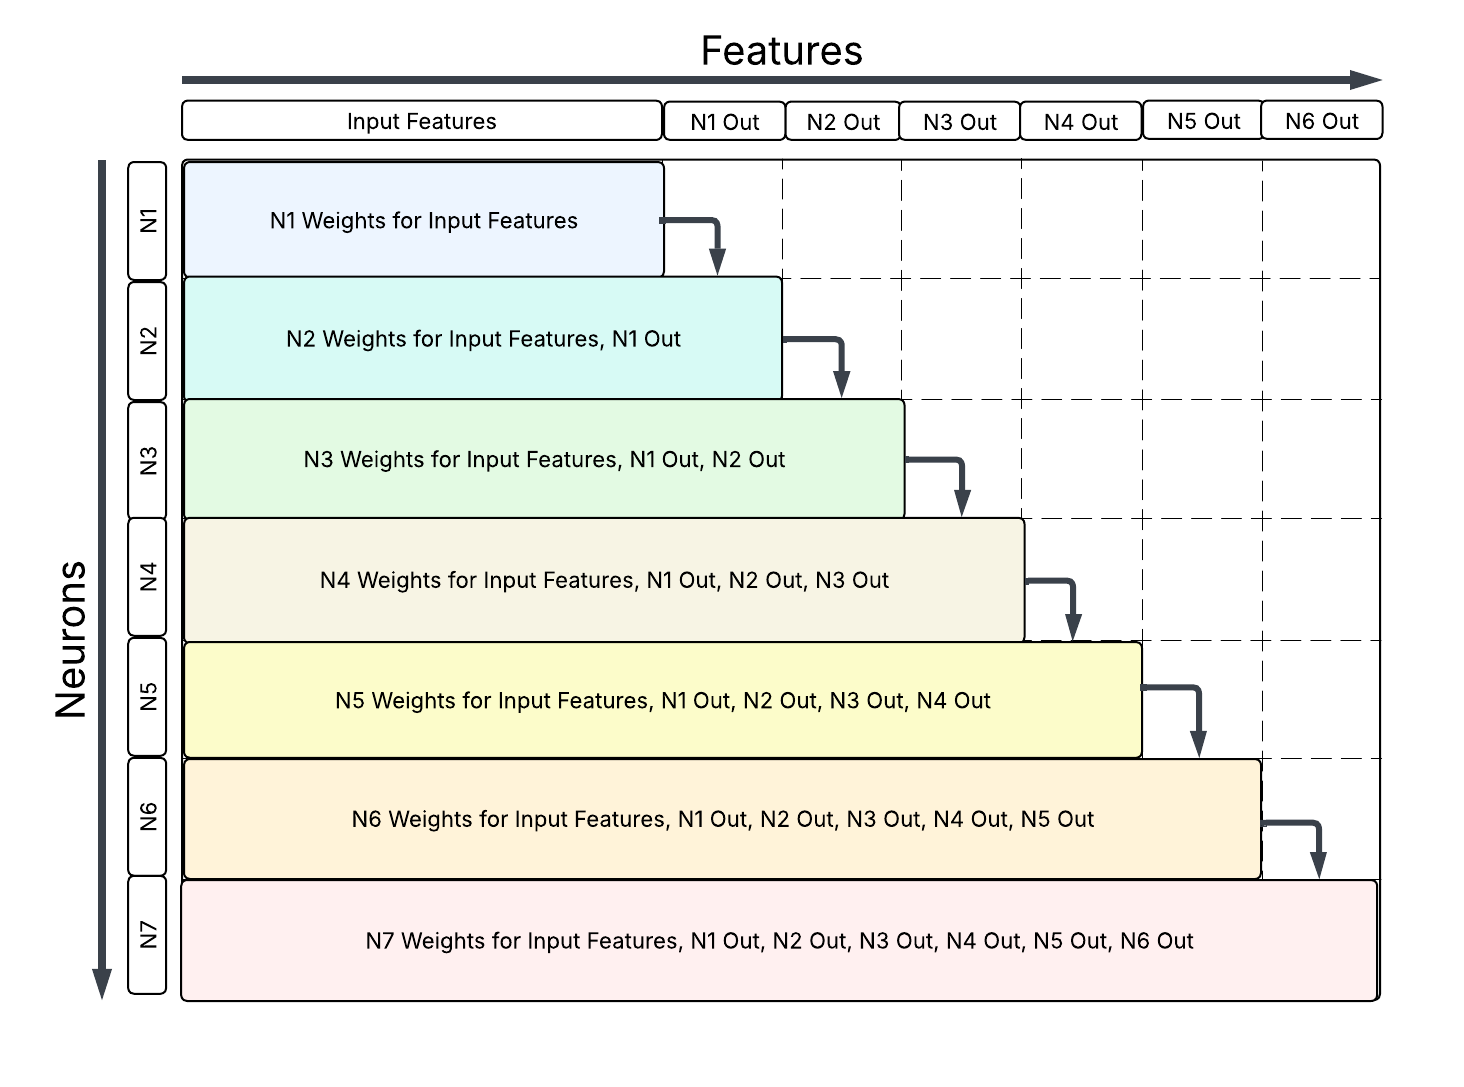
\includegraphics[width=0.7\textwidth]{Figures/Methodology/Neuron_Based_Maximal_SPN_Weights.png}
\caption{Illustration of a sequential Maximal SPN.}
\label{fig:seqMaxSpn}
\end{figure}

\subsection{Sequential Representation with Shared Input}
This approach is identical to the previous one, with the key difference being that instead of storing inputs temporarily, neurons index slices from an input variable shared across the entire network. This indexing does not add significantly to the time complexity but optimizes it by eliminating redundancy.

Time Complexity: O(n).

Space Complexity: O(d * n²).


\subsection{Block-based Representation with Partial Outputs and Shared Input}

When considering the lower triangular weight matrix and visualizing vertical lines at the edge of each neuron’s weight vector, we see the formation of blocks within the matrix. The largest block contains the weights corresponding to the input features, and subsequent blocks contain the weights for the output of each neuron.
 
Rather than processing each neuron’s weight vector individually, this approach processes the network one block at a time. The top-most neuron’s forward pass is completed first, followed by calculating partial outputs for the remaining neurons. This method improves the time complexity by prioritizing the heaviest calculations (typically when the hardware is under lower load), and adds slight parallelization, as an input value is accessed only once, rather than repeatedly in a sequential approach.

This method is both energy and time-efficient, offering significant improvements over the previous approaches.

Time Complexity: O(n).

Space Complexity: O(d * n²).

\begin{figure}[ht]
\centering
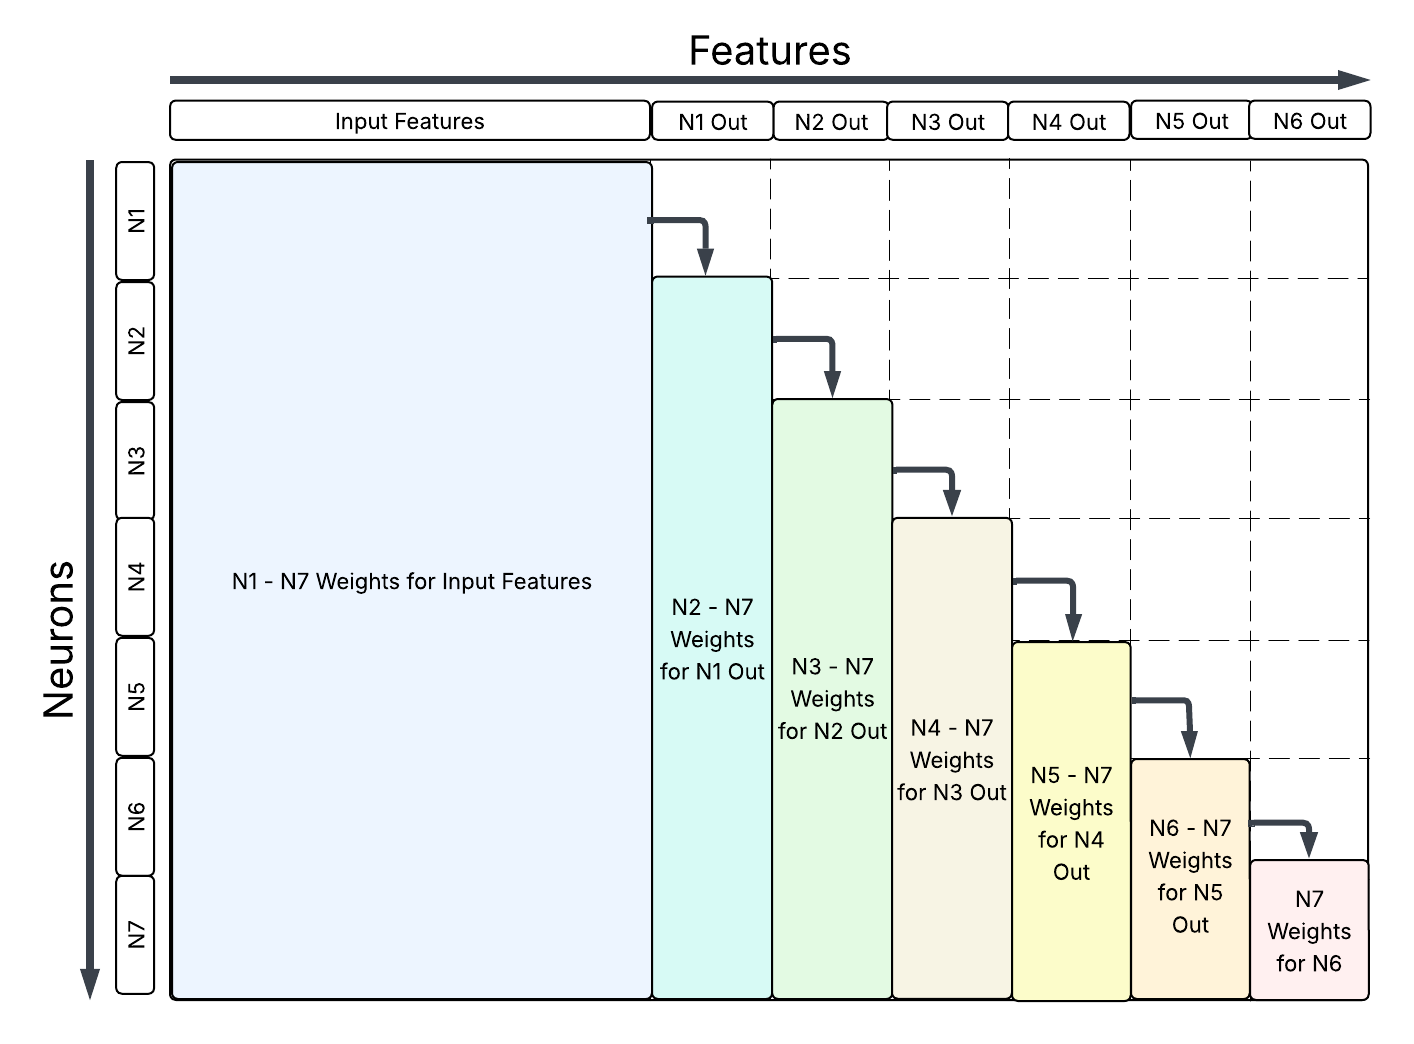
\includegraphics[width=0.7\textwidth]{Figures/Methodology/Block_Based_Maximal_SPN_Weights.png}
\caption{Illustration of a block based Maximal SPN.}
\label{fig:blockMaxSpn}
\end{figure}

\section{Free Weights}

When projecting traditional MLPs onto a lower triangular matrix, we notice weight blocks isolated both vertically and horizontally. These isolated weights represent the independent layers in traditional MLPs. The right side of the matrix defines the time complexity of the forward pass; the more layers present, the longer the processing time. However, the left side of the matrix contains Free Weights, zeroed-out weights that do not contribute to time complexity.
 
Using free weights in traditional MLPs is similar to concatenating the output of a layer to its input before passing it to the next layer. This method increases the space complexity of the MLP to O(n²) while keeping the time complexity at O(l), where l is the number of layers. A major advantage of this approach is that subsequent layers can learn features based on both the input and the features from other previous layers, enabling the network to learn more complex patterns.

\begin{figure}[ht]
\centering
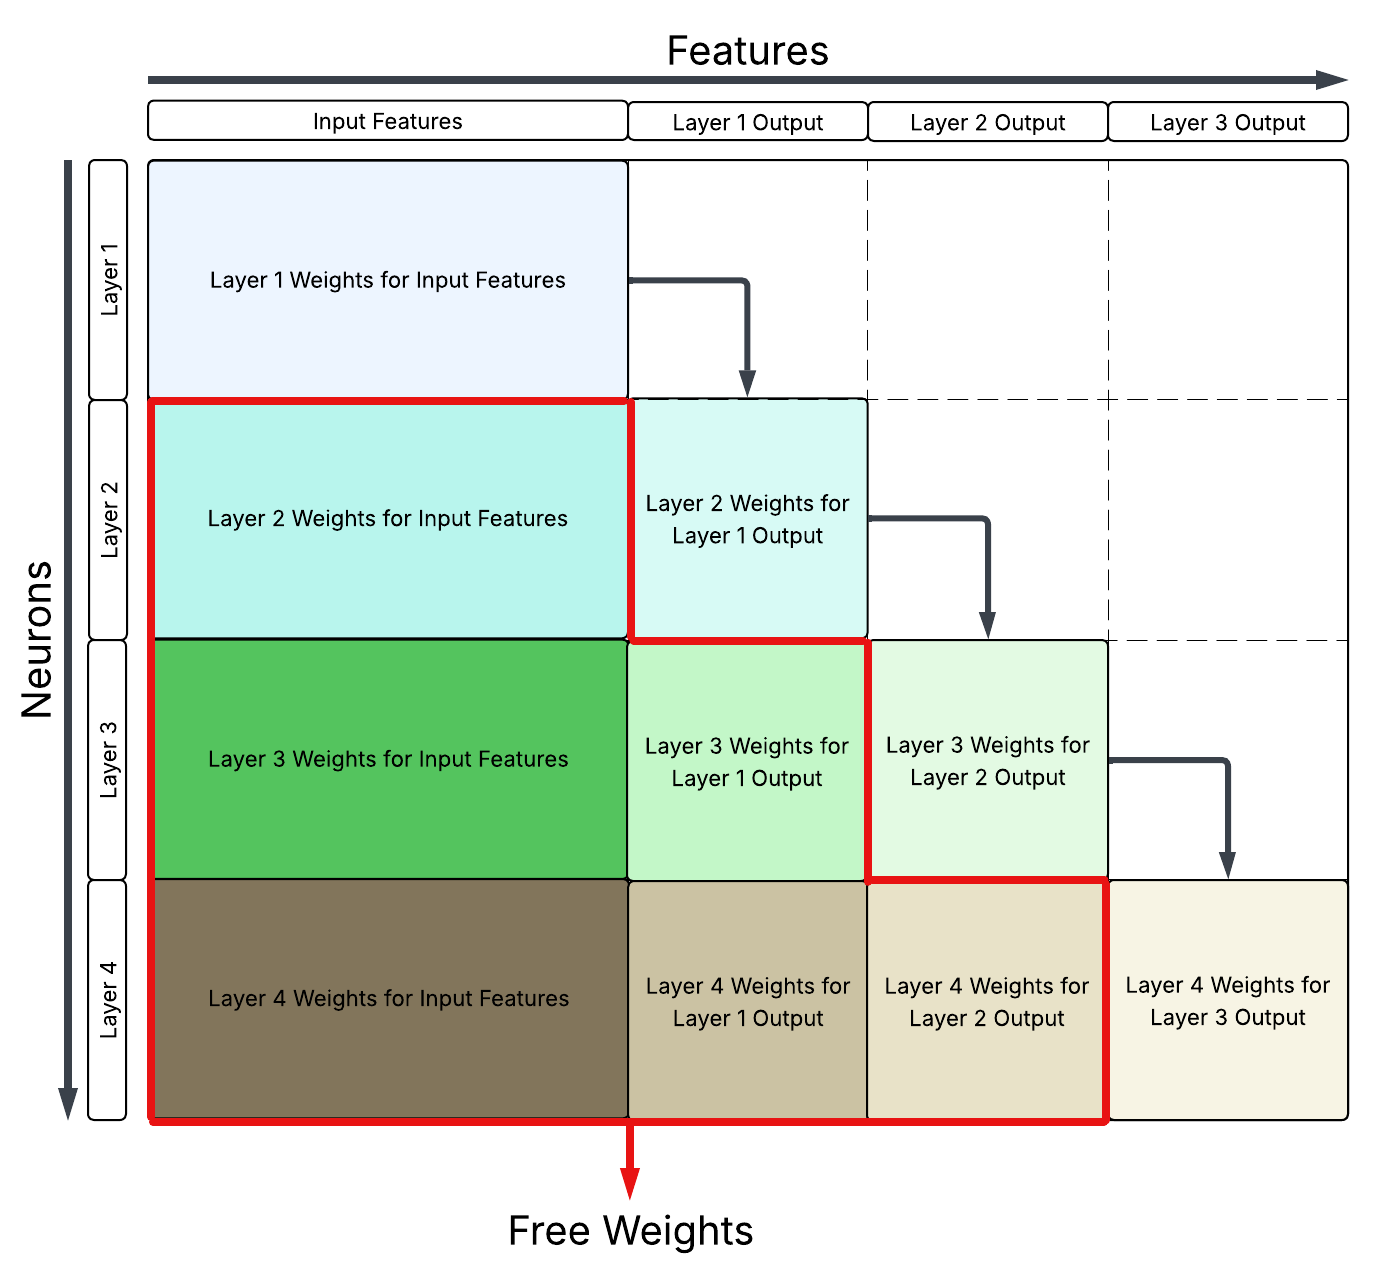
\includegraphics[width=0.7\textwidth]{Figures/Methodology/Free_Weights_SPN_Weights.png}
\caption{Illustration of a traditional MLP with Free Weights.}
\label{fig:fwSpn}
\end{figure}

\section{Minimal SPNs}

While maximal SPNs maximize the number of connections in a perceptron network, they come with the trade-off of significantly increasing the time complexity from O(l) (where l is the number of layers) to O(n) (where n is the total number of neurons). Since l << n in most perceptron networks, this added time complexity becomes a significant challenge.
On the other end of the spectrum, Minimal SPNs seek to minimize the number of blocks in the SPN framework. There are two possibilities:

1.	If the total number of neurons is equal to the output size (n == o), only one block is needed, equivalent to a single MLP layer of size n.

2.	If the total number of neurons exceeds the output size (n > o), the network must have at least two layers: one layer of size n - o for the input, and a second layer of size o that takes both the input and the output of the first layer.
 
Minimal SPNs provide the best time complexity of O(1) and the best space complexity of O(n²).

\begin{figure}[ht]
\centering
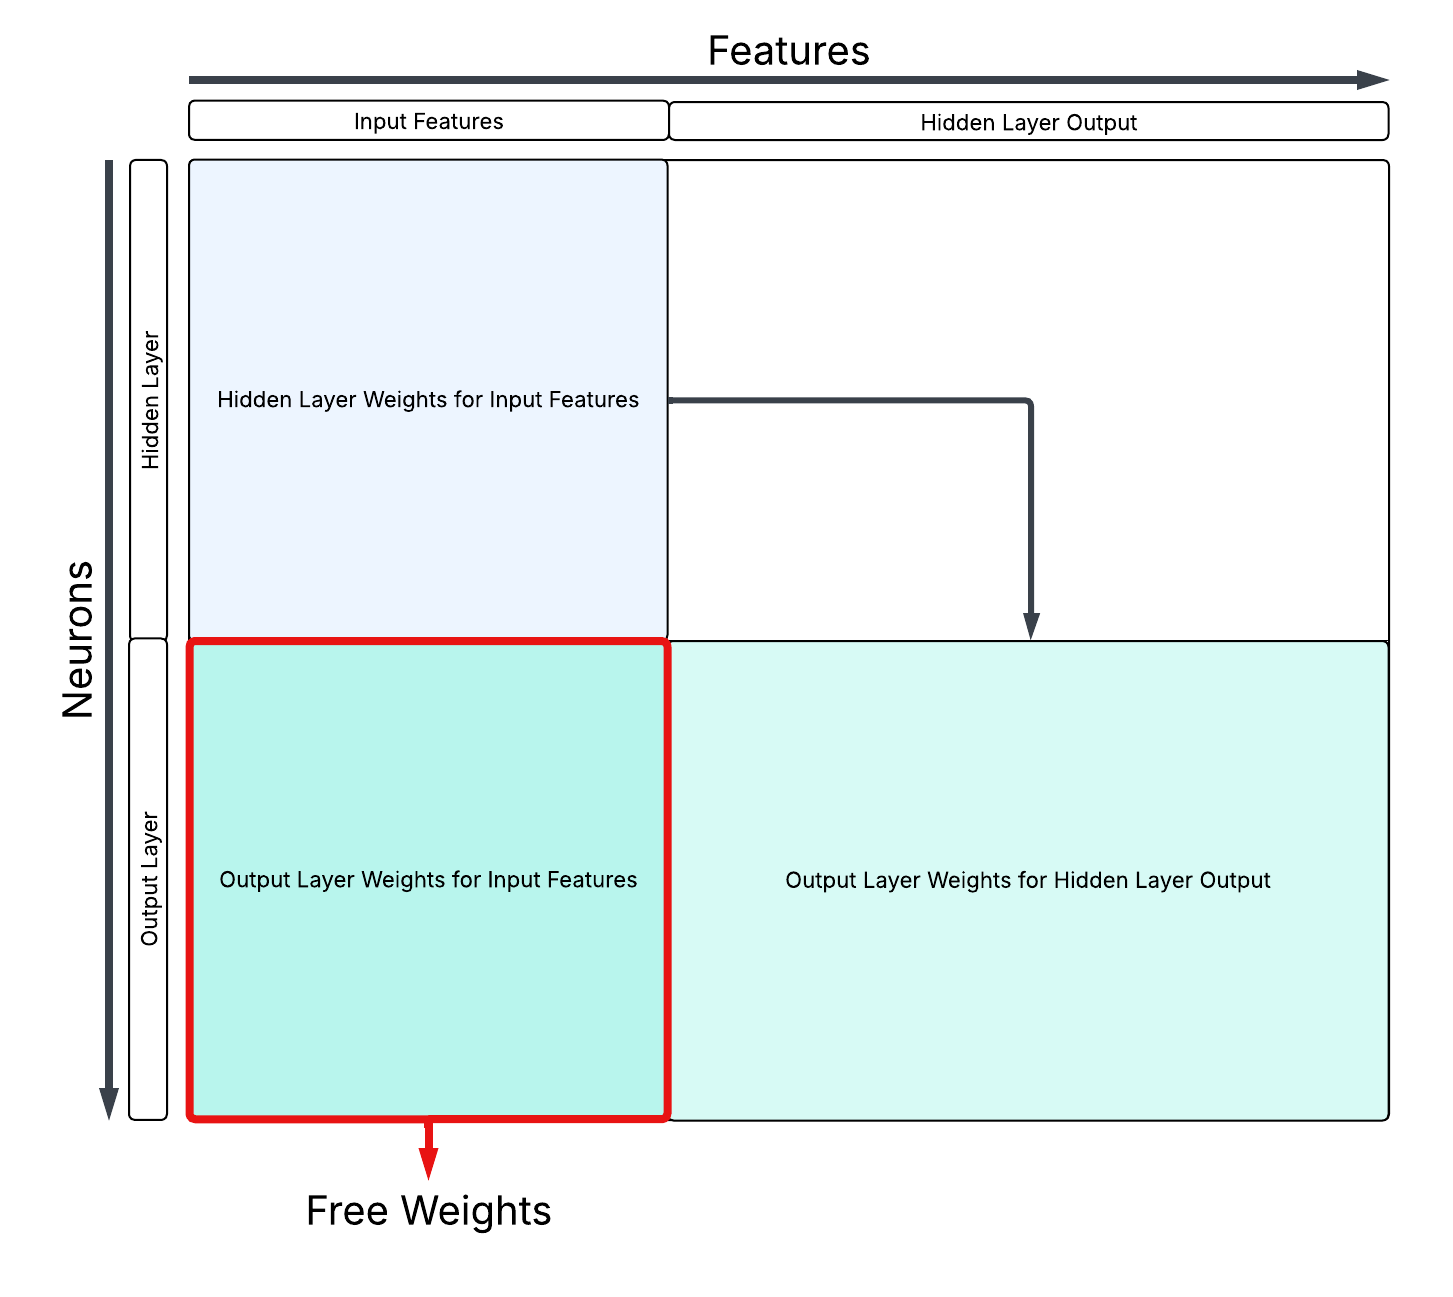
\includegraphics[width=0.7\textwidth]{Figures/Methodology/Minimal_SPN_Weights.png}
\caption{Illustration of a Minimal SPN.}
\label{fig:minSpn}
\end{figure}

\section{Maximal SPNs with Pruning}

The final approach to improving SPN efficiency is pruning, inspired by the lottery ticket hypothesis. According to this hypothesis, there exists a smaller subnetwork within a neural network that can perform similarly to the original network if trained on the same dataset. The process involves training the parent network briefly (e.g., for one epoch), pruning the network slightly, and then resetting the remaining weights to their original values before repeating the first step for a desired number of iterations, until the network reaches a desired size. Then, the best performing pruned version of the network is trained for the complete duration.
 
This approach is applied to Maximal SPNs by zeroing out weights along the right edge of the lower triangular matrix. This pruning allows some neurons to share the same right-side edges, enabling parallel processing. The time complexity of the network is improved to O(l), where l is the number of vertical edges on the right side of the SPN matrix. Additionally, this method can reduce the space complexity by up to 90\%, making it highly efficient.